% \begin{figure}
%     \centering
%     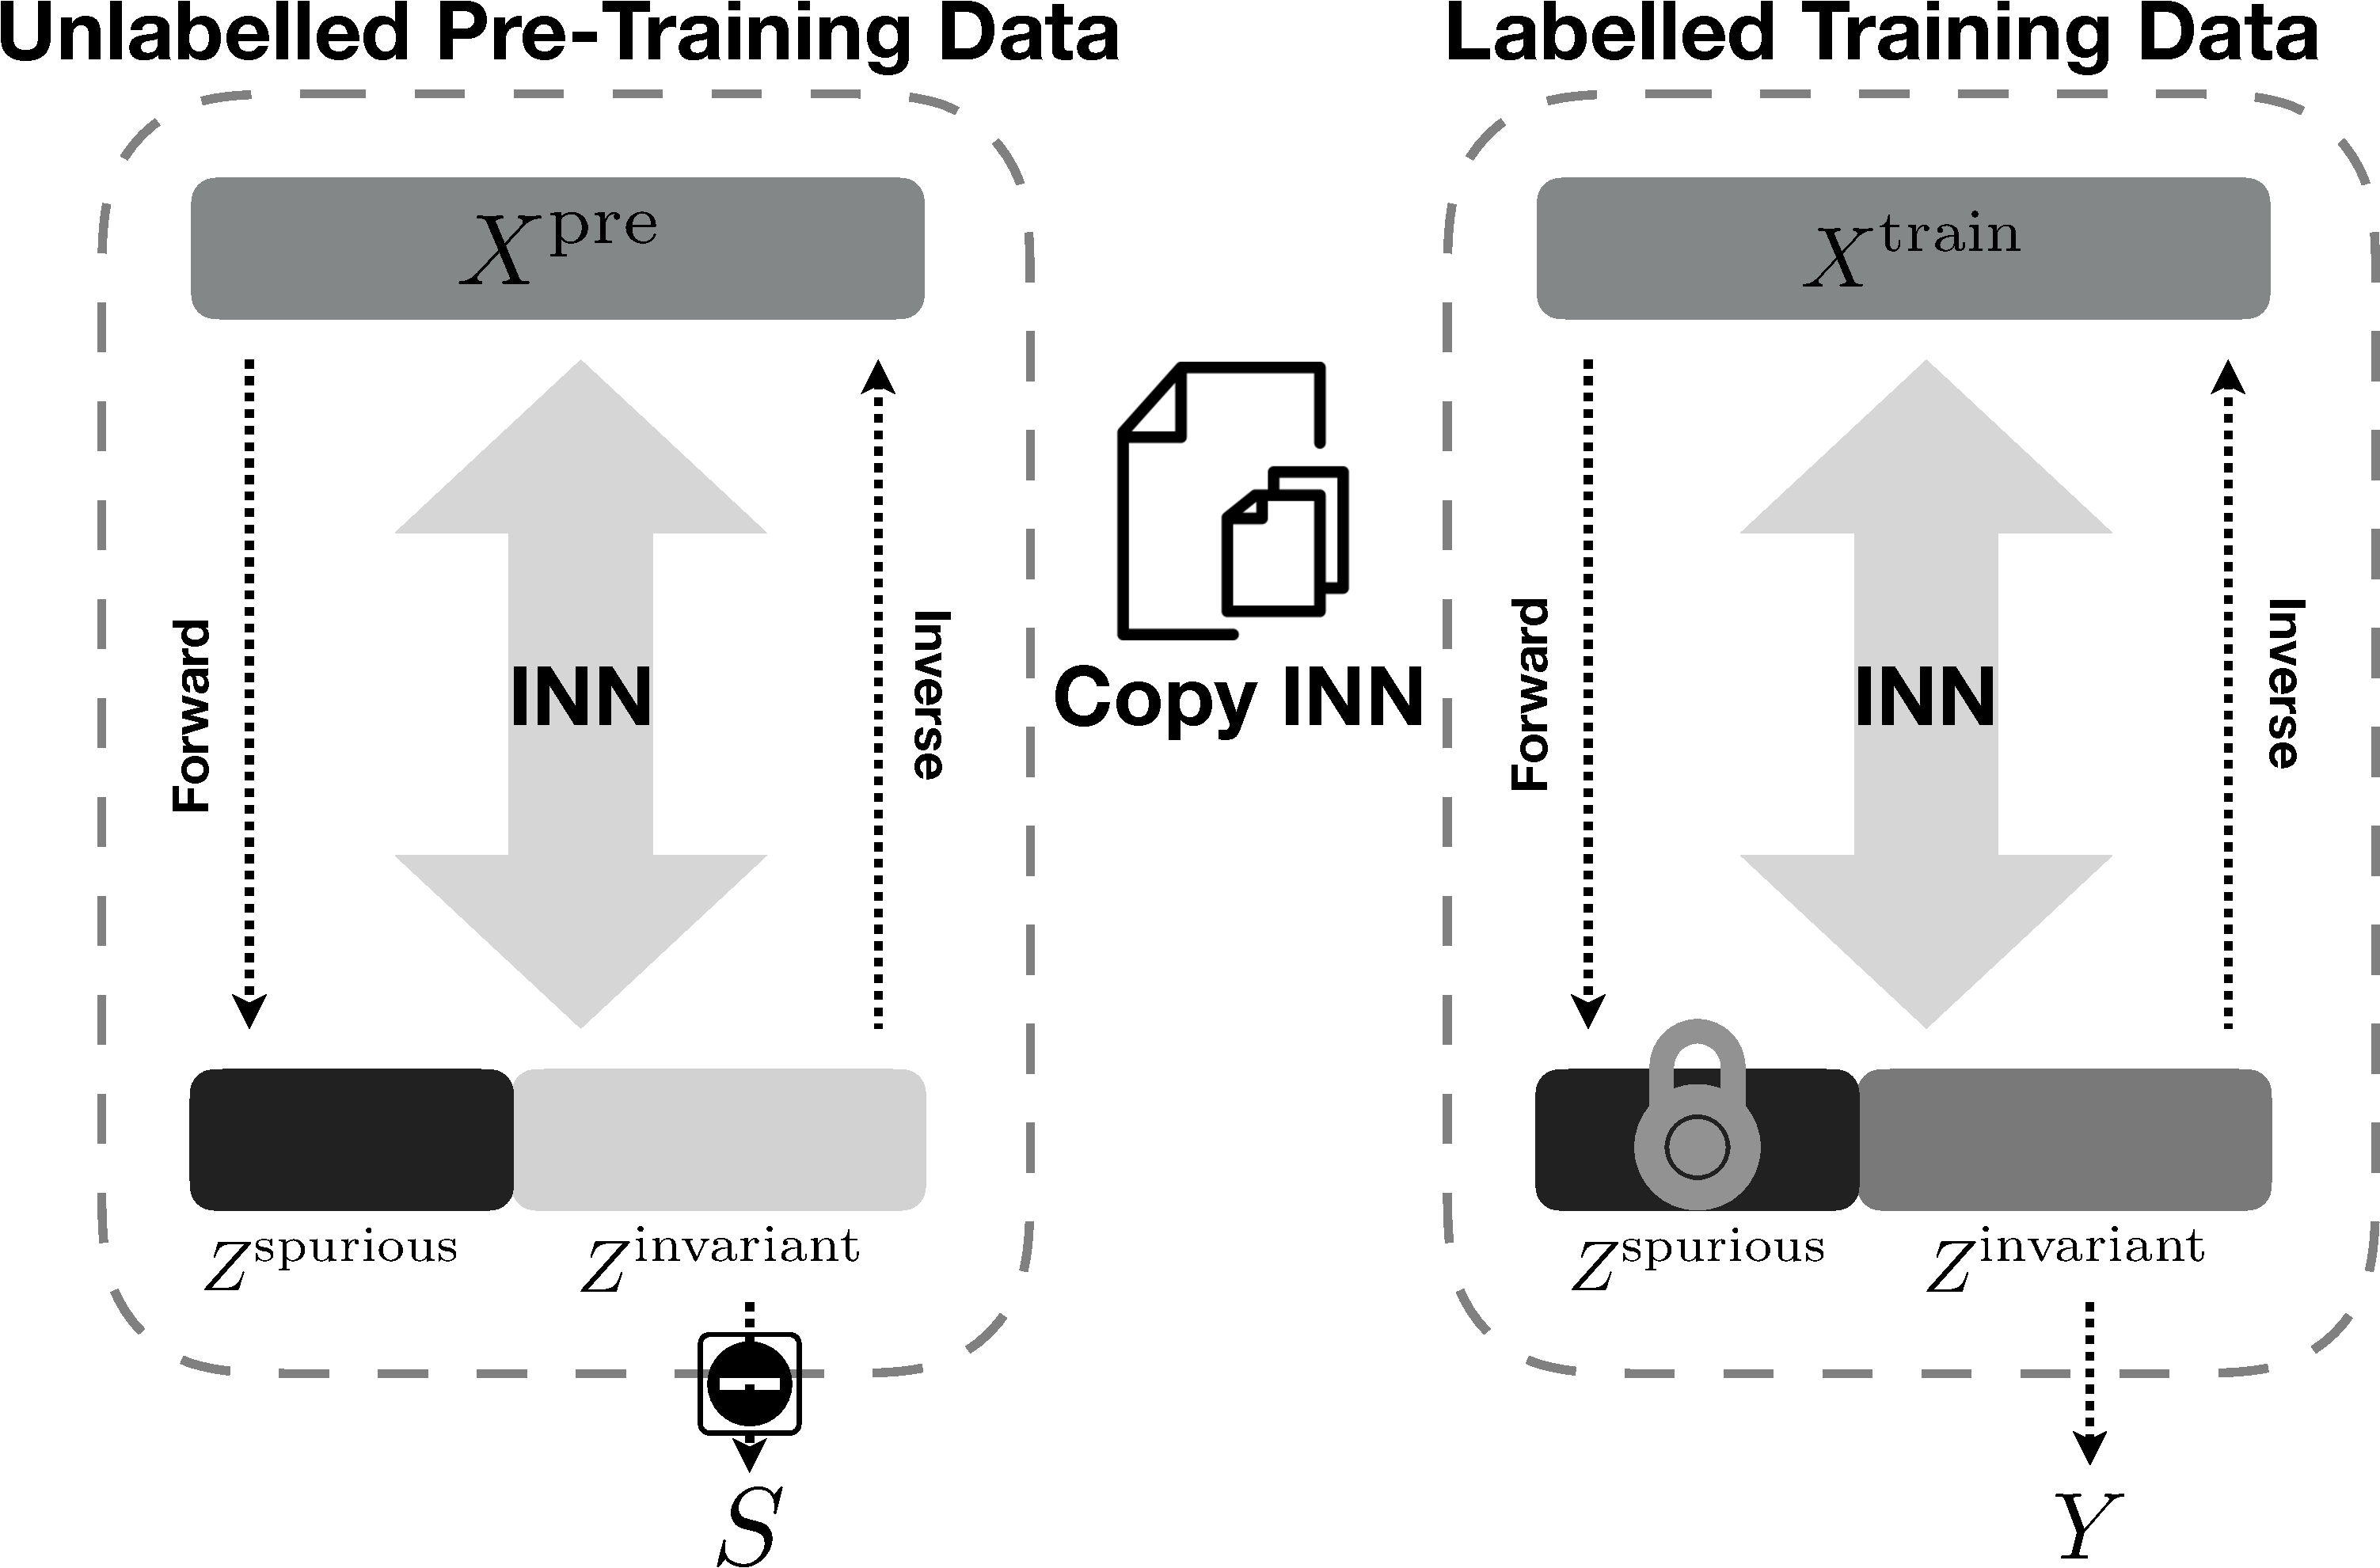
\includegraphics[width=0.4\textwidth]{nifr/Figures/diagram.pdf}
%     \caption{Training procedure using the cFlow model for illustrative purposes.}%
%     \label{fig:training_diagram}
% \end{figure}
\begin{figure*}[tb]
    \centering
    \hfill
    \subfloat[cFlow model.]{%
        \scalebox{0.4}{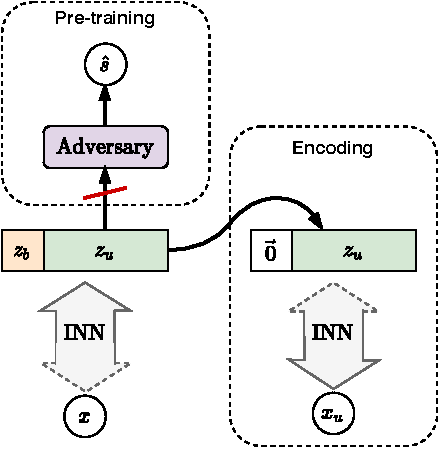
\includegraphics[width=\textwidth]{nifr/Figures/inn_diagram_u.pdf}}%
        \label{fig:inn_diagram}
    }
    \hfill
    \subfloat[cVAE model.]{%
        \scalebox{0.5}{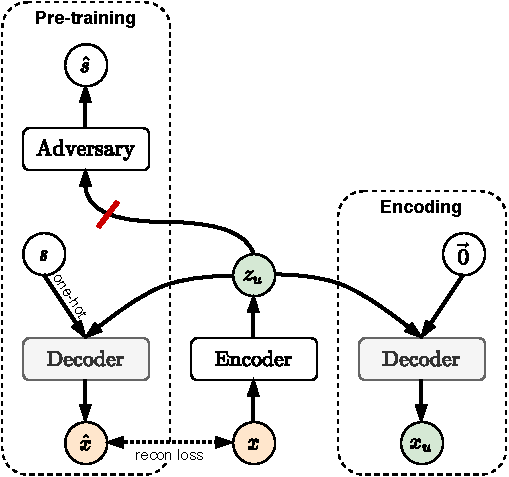
\includegraphics[width=\textwidth]{nifr/Figures/cvae_diagram_u.pdf}}%
        \label{fig:cvae_diagram}
    }
    \hfill
    \caption{
          High-level diagram showing the training procedure for our proposed models (a) \ac{cFlow}
          and (b) \ac{cVAE} models.
        %
          Here, $x$ denotes the input, $s$ the sensitive attribute, $z_u$ the de-biased (invariant
          to \(s\)) representation, and $x_u$ the de-biased version of the input in the data domain
          (i.e. the pre-image of \(z_u\) under the models, either by exact (\ac{cFlow}) or
          approximate (\ac{cVAE}) inversion). 
        %
          The red bar bisecting the arrows between the adversary and \(z_u\) indicates a
          Gradient-Reversal Layer (GRL), as per \citet{ganin2016domain}; $\vzero$ represents the
          null-sampling operation which amounts to setting \(z_b\) or \(s\) to the zero-vector for
          the \ac{cFlow} and \ac{cVAE} models, respectively.
        %
          Null-sampling (shown on the right of each sub-figure) -- the procedure generating the
          de-biased input \(x_u\) -- is only conducted for visualisation purposes (i.e. no
          gradients ever flow through the operation), though this may be useful during training in
          order to diagnose pathologies; during training the ground-truth \(s\) label is one-hot
          encoded (giving \(e_s\), per Eq.~\ref{eq:objectivepractical}) and fed as input to the
          decoder, the output of which (\( \hat{x} \)) is used for computing the \ac{cVAE}'s
          reconstruction (\ac{MI}) loss. 
        %
          Note that the dotted arrow heads in (a) denote an implicit operation; during training of
          the \ac{cFlow} model, we need only compute the inverse (\(x \mapsto z_u\)) model due to
          its bijectivity; for generating \(x_u\), however, it is necessary to run the model both
          ways with null-sampling as an intermediary intervention on the latent space.
        %
        % CORRECTED: 
        % 1. Could move closer to where referenced in the text and could refer to it more in the
        % text.
        %
        % 2. Maybe add to figure as discussed in the viva -- this refers to the clarity of the
        % decoder's involvement during training (only the encoder is involved in the
        % invariance-learning procedure) and of the involvement of null-sampling at this time (i.e.
        % there is none -- the decoder is fed the ground-truth labels and null-sampling is only
        % applied at inference-time).
        %
        %$ 3. Could also add to the caption and maybe also in the text where you describe the
        %figure. No page constraints any more!
    }%
    \label{fig:model-diagrams}
\end{figure*}

